\chapter{Namens- und Verzeichnisdienste}

\section{Namensdients}
Ein \textbf{Namensdienst} bildet einen (menschenfreundlichen) Namen zu einem Objekt ab. Beispielsweise assoziiert das Dateisystem einen Dateinamen zu einem \emph{Filehandler} und der DNS einen Namen zu einer IP-Adresse. Das \textbf{Namenssystem} beschreibt den Syntax, welcher für die Namen befolgt werden muss. Das Unix-Dateisystem schreibt vor, dass der Name immer mit einem '/' beginnen muss (/etc/hosts). Im DNS werden Objekte mit dem Punkt-Operator (www.20min.ch) deklariert. Der Assoziations-Vorgang zwischen Namen und Objekt wird \textbf{binding} genannt. Typischen Namensdienste: RMI Registry, CORBA Naming Service.

\section{Verzeichnisdienst}
Der \textbf{Verzeichnisdienst} kann im Gegensatz zu einem reinen Namensdienst etwas mehr. Es werden nicht nur Bindings erstellt, sondern es können auch Verzeichnisdienst spezifische Attribute zum Objekt abgelegt werden. Auf Basis diesen Attributen kann im Verzeichnis gesucht werden. Typischer Verzeichnisdienst: LDAP.

\section{JNDI}
Das Java Naming und Directory Interface (JNDI) ist ein Java-API für Namens- und Verzeichnisdienste. Über die Schnittstelle können Daten- und Objektreferenzen anhand eines Namens abgelegt und von Nutzern des API wieder abgerufen werden. Dieses API ist ein sogenanntes Server Provider Interface (SPI), damit können Hersteller eigene Lösungen bauen. Über JNDI werden die meisten bekannten Dienste unterstützt, wie: LDAP, DNS, NIS (Network Information Service), CORBA (Common Object Request Broker Architecture), Dateisystem, RMI. Wir dürfen froh sein, dass wir mit EJB 3.x arbeiten. Davor mussten alle Referenzen auf Ressourcen im Deployment Deskriptor verwaltet werden und anschliessend mittels JNDI-Lookups in den EJBs programmiert werden. Es gab weder Annotationen noch die mächtigen Mechanismen der Dependency Injection.

\subsection{API}
Das API beinhaltet folgendes:
\begin{itemize}
	\item Mechanismus zum Binden von Objekten an einen Namen
	\item Methoden für den Abruf von Informationen anhand eines Namens
	\item Clients können über Änderungen informiert werden, dies ist mittels einem Ereigniskonzept umgesetzt
	\item Spezielle Erweiterungen für LDAP-Funktionalitäten
\end{itemize}

\subsection{Architektur}
Am einen Ende ist das JNDI und am anderen Ende die Server Provider Implementation, welche über das Service Provider Interface spezifiziert ist. Der Naming-Manager ist das Verbindungsstück zwischen API und SPI.

\begin{figure}[h!]
\centering
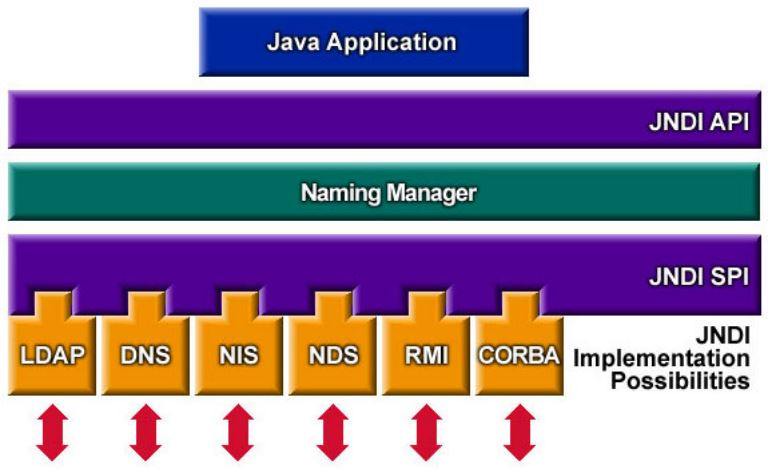
\includegraphics[width=0.5\linewidth]{fig/jndi-architecture}
\caption{JNDI Architektur}
\label{fig:jndi-architecture}
\end{figure}

\subsection{Packages}
\begin{description}
	\item[javax.naming:] Definiert ein Naming Context Interface, welches
	das Core-Interface für lookups, bind/unbind, renaming für
	Objekte und erzeugen/löschen von Subkontext darstellt.
	\item[javax.naming.directory:] Erweitert das Naming-Package mit den
	Zugriffen auf Namens Services. Erlaubt das Abholen von
	Attributen assoziert mit Objekten gespeichert im Directory.
	\item[javax.naming.event:] Unterstützt die Event Notifikation in
	Directory Services. Es gibt Events und Listeners.
	\item[javax.naming.ldap:] Erweitert das javax.naming.directory Packet
	mit erweiterten Operation Controls. Auf Basis von LDAPv3.
	\item[javax.naming.spi:] Unterstützt die Entwickler von
	Namensdiensten bei der Implementierung von Services. 
\end{description}

\subsection{JNDI-Lookup}
Beim \textbf{Lookup} (Nachschlagen) wird den Name verwendet um das korrespondierende Objekt zu ermitteln. 

\begin{lstlisting}[language=Java, caption=Beispiel programmatischer EJB-Lookup]
try {
	Friend friend = (Friend) new InitialContext().lookup("java:comp/env/myFriend");
} catch (NamingException e) {
	e.printStackTrace();
}
\end{lstlisting}

\begin{figure}[h!]
\centering
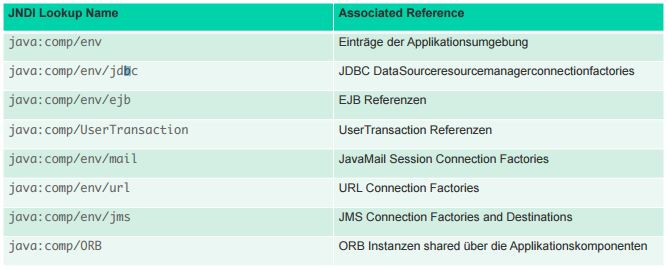
\includegraphics[width=0.7\linewidth]{fig/jndi-lookups}
\caption{JNDI Lookups und assoziierte Referenzen}
\label{fig:jndi-lookups}
\end{figure}

\subsection{Externe JNDI Ressourcen}
Java EE Applikationen benötigen oft Zugriff auf Ressourcen, welche in einem externen JNDI Repository gespeichert sind. Beispielsweise können Objekte in einem LDAP Server gespeichert werden. Dazu muss die Verbindung zum LDAP Server wie in Listing \ref{lst:verbindung-ldap} konfiguriert werden.

\begin{lstlisting}[caption=Verbindung zum LDAP, label=lst:verbindung-ldap]
<external-jndi-resource jndi-name="test/myBean" jndi-lookup-name="cn=myBean" res-type="test.myBean" factory-class="com.sun.jndi.ldap.LdapCtxFactory">
	<property name="PROVIDER-URL" value="ldap://ldapserver:389/o=myObjects" />
	<property name="SECURITY_AUTHENTICATION" value="simple" />
	<property name="SECURITY_PRINCIPAL", value="cn=joeSmith, o=Engineering" />
	<property name="SECURITY_CREDENTIALS" value="changeit" />
</external-jndi-resource></resources>
\end{lstlisting}

\section{LDAP}
Dass \textbf{Lightweight Directory Access Protocol} ist mehr als nur ein Protokoll. Es beinhaltet vier Modelle:
\begin{itemize}
	\item Informations-Modell
	\item Namens-Modell
	\item Funktionales-Modell
	\item Sicherheits-Modell
\end{itemize}
Es gibt APIs für die unterschiedlichsten Programmiersprachen (C-API, Java (JNDI), Perl-LDAP, PHP LDAP und auch Unix-CMD). Das LDIF (LDAP Data Interchange Format) dient um Informationen aus dem Verzeichnisdienst in einem ASCI-basierten Dateiformat darzustellen.

\begin{lstlisting}[caption=Beispiel LDIF]
dn: uid=zajoho, ou=people, dc=el, dc=campus, dc=intern

objectclass: top
objectclass: person
cn: Bruno Joho
givenname: Bruno
uid: zajoho
mail: bruno.joho@hslu.ch
\end{lstlisting}


\begin{lstlisting}[caption=Beispiel LDIF Update]
dn: uid=zajoho, ou=people, dc=el, dc=campus, dc=intern

changetype: modify
replace: givenname
	givenname: Bruno Joho
	givenname: Bruno Joho Teacher
add: mail
	mail: bjoho@HSLU.ch
\end{lstlisting}

\subsection{Geschichte}
LDAP hat seinen Ursprung an der Universtiät von Michigan (UMich) und wurde erstmals in einem RFC vorgeschlagen. LDAP soll eine alternative zum DAP darstellen, welches X.500 (beschreibt Aufbau eines Verzeichnisdienstes) vollständig implementierte mit einem ganzen OSI/ISO Stack. LDAP verwendet dabei nur einen TCP/IP Stack.

\subsection{Unterschiede zur DB}
\begin{itemize}
	\item Lese/Schreib Verhältnis
	\item Erweiterbarkeit
	\item Verteilbarkeit
	\item Replizierbarkeit
	\item Geschwindigkeit
	\item Standardisierung 
\end{itemize}

\subsection{Modelle}

\subsubsection{Informationsmodell}
Das Informationsmodell definiert Datentypen und Grundeinheiten der Informationen, die im Verzeichnis gespeichert werden sollen. Die Grundeinheit ist ein Entry der aus mehreren Attributen besteht. Attribute haben einen Typ und dürfen einen oder mehrere Werte annehmen. Attribute können vom Benutzer (normale Attribute) oder vom System (Operationale Attribute z.B. Timestamp) modifiziert werden. Attribute können auch Bedingungen (Constraints) haben z.B. Länge der Zeichenkette.

\subsubsection{Namensmodell}

Das Namensmodell spezifiziert die Struktur der Daten. Die Datenstruktur ist ein hierarchischer Baum mit Wurzeln, Zweigen und Blättern. Dieser Baum wird auch Directory Information Tree (DIT) genannt. Die Wurzel (root, suffix) ist das oberste Datenobjekt, unter ihm verzweigen sich die höheren Strukturen. Oft wird der Unternehmensnamen als Wurzerl definiert (\emph{o=css}). Personen oder Gruppen können dann darunter angelegt werden (\emph{ou=people,o=css} oder \emph{ou=groups,o=css}). Ein einzelnes Objekt wird durch den Distinguished Name (DN) eindeutig identifiziert (\emph{uid=tdsuter,ou=people,o=css}). Dieser setzt sich aus mehreren Relative Distinguished Names (RDN) zusammen. Eine anderen Namen für DN ist der canonical Namen, wobei der Pfad mit Slashes getrennt wird (\emph{css/people/tdsuter}). Einige bekannte Abkürzungen:

\begin{itemize}
	\item cn = common name
	\item ou = organizational unit
	\item st = state
	\item c = country
	\item mail = e-mail
	\item dc = domain component
\end{itemize}

\begin{figure}[h!]
\centering
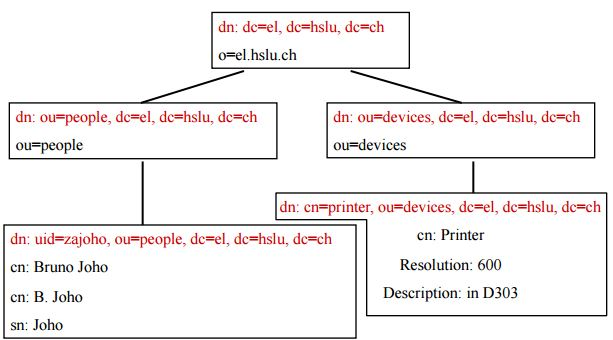
\includegraphics[width=0.7\linewidth]{fig/ldap-namens-modell}
\caption{Namens-Modell}
\label{fig:ldap-namens-modell}
\end{figure}

\subsubsection{Sicherheitsmodell}

Das Sicherheitsmodell dient dazu Informationen im Verzeichnis vor unautorisiertem Zugriff zu schützen. Für die Authentifizierung schickt ein Benutzer über einen Client einen DN und ein Password. Der Server sucht den Eintrag aus dem Verzeichnis heraus und authentiziert den Client, wenn das gegebene Passwort richtig ist. SSL und TLS sind Konzepte, um Daten zu verschlüsseln. Leider bietet LDAP kein allgemeines Access Control Model (Art und Weise wie Zugriffsrechte beschrieben werden), sondern nur eine eigene Access Control Instruction.

\subsubsection{Funktionale Modell}

Das Funktionale Modell beschreibt die möglichen Operatione mit den entsprechenden Parameter. Es gibt \textbf{Interrogation Operationen}, welche zur Abfrage dienen. Es gibt keinen Read-Operator sondern nur einen Search, welcher bis zu 8 Parameter kennt. Dazu gibt es \textbf{Update Operationen} (Hinzufügen, Löschen, Verändern). Zu guter Letzt existieren die \textbf{Authentcation \& Control Operations} (Bind, Unbind, Abandon).